\documentclass[12pt, a4paper]{article}

% Paquetes esenciales
\usepackage[utf8]{inputenc}
\usepackage[T1]{fontenc} % <--- Soluciona los caracteres extraños
\usepackage{lmodern}     % <--- Fuente vectorial compatible con T1
\usepackage[spanish,es-nodecimaldot]{babel}
\usepackage[margin=2.5cm]{geometry}
\usepackage{graphicx}
\usepackage{xcolor}
\usepackage{tcolorbox}
\usepackage{enumitem}
\usepackage{hyperref}
\usepackage{titlesec}
\usepackage{caption}
\usepackage{fontawesome5}

% Configuración de colores institucionales
\definecolor{primary}{RGB}{31, 106, 165}
\definecolor{warning}{RGB}{200, 50, 50}
\definecolor{success}{RGB}{16, 74, 32}

% Configuración de hipervínculos
\hypersetup{
    colorlinks=true,
    linkcolor=primary,
    urlcolor=primary
}

% Formato de títulos
\titleformat{\section}{\Large\bfseries\color{primary}}{}{0em}{}[\titlerule]
\titleformat{\subsection}{\large\bfseries\color{darkgray}}{}{0em}{}

% Estilos de cajas de advertencia e información
\newtcolorbox{advertencia}{colback=warning!5!white, colframe=warning, fonttitle=\bfseries, title=\faExclamationTriangle\ IMPORTANTE}
\newtcolorbox{nota}{colback=primary!5!white, colframe=primary, fonttitle=\bfseries, title=\faLightbulb\ Nota Técnica}

\begin{document}

% Portada / Encabezado
\begin{center}
    {\Huge \textbf{\color{primary} Manual de Configuración}}\\[0.5cm]
    {\Large Sistema de Reja Automatizada - 10 Cedros}\\[0.5cm]
    {\normalsize Documento de uso exclusivo para residentes}
    \vspace{0.5cm}
    \hrule
\end{center}

\vspace{0.5cm}

Este manual le guiará paso a paso para configurar la aplicación móvil y vincular su acceso autorizado a la reja del fraccionamiento. Le tomará aproximadamente 3 minutos completar este proceso.

\section*{Obtener la aplicación y registrarse}

\begin{enumerate}[label=\textbf{Paso \arabic*:}, leftmargin=*]
    %PASO 1
    \item \textbf{Instalar la aplicación oficial}\\
    \textbf{Busque y descargue} la aplicación \textit{Smart Life} (ícono de casa azul de \textit{Volcano Technology Limited}) en la tienda de su dispositivo. Puede acceder directamente con los siguientes links según su celular:
    \begin{itemize}
        \item \textbf{Play Store:} \href{https://play.google.com/store/apps/details?id=com.tuya.smartlife}{Descargar aquí}
        \item \textbf{App Store:} \href{https://apps.apple.com/us/app/smartlife-smart-living/id1115101477}{Descargar aquí}
    \end{itemize}
    
    \begin{center}
        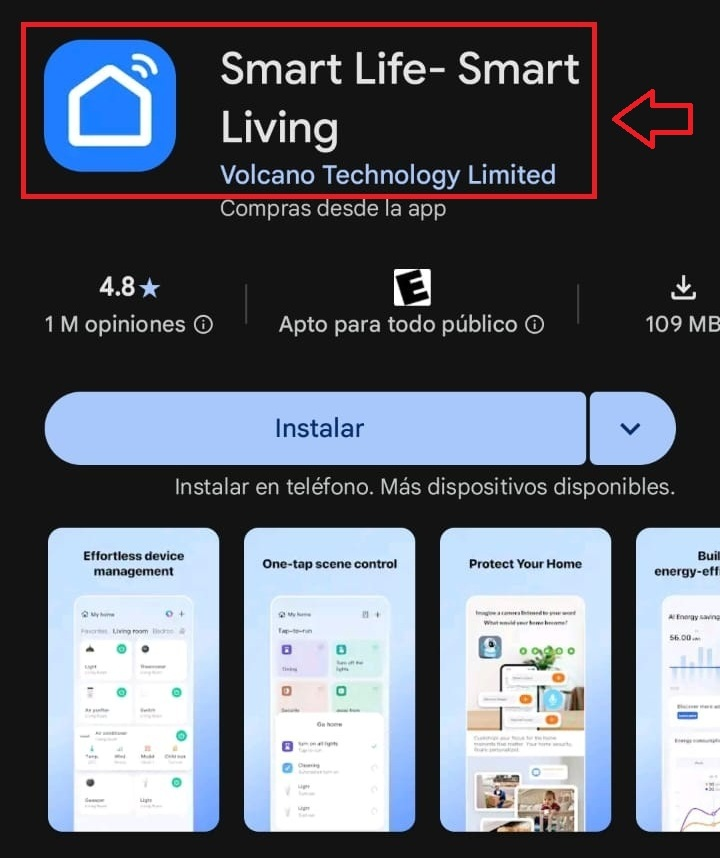
\includegraphics[width=0.4\textwidth]{Paso1.jpeg}
    \end{center}

    \newpage
    %PASO 2
    \item \textbf{Abrir la app por primera vez}\\
    \textbf{Abra} la aplicación. \textbf{Presione} el botón blanco \textit{Crear cuenta nueva}.\\
    Si usted tiene una cuenta existente, entre a la app \textbf{asegurándose} de entrar con el mismo correo que envió al momento de realizar su pago. De lo contrario, la reja no abrirá.
    
    \begin{center}
        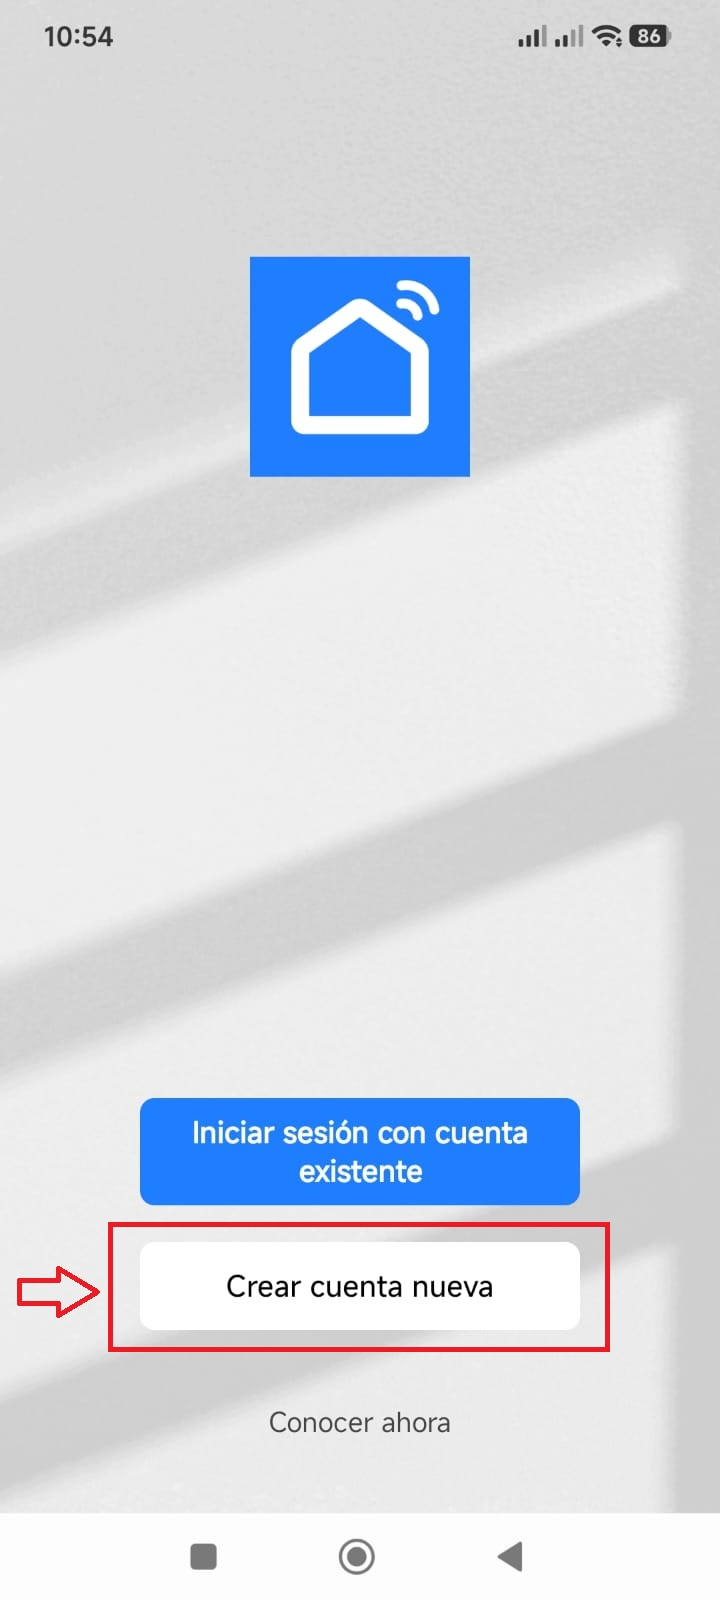
\includegraphics[width=0.4\textwidth]{Paso2.jpeg}
    \end{center}
\end{enumerate}

\newpage
\section*{Vincular su correo vecinal}

\begin{advertencia}
    El sistema de la reja está vinculado a la base de datos del administrador. Si utiliza un correo distinto al que envió al hacer su pago, la reja no abrirá.
\end{advertencia}

\begin{enumerate}[label=\textbf{Paso \arabic*:}, leftmargin=*, resume]
    %PASO 3
    \item \textbf{Escribir su correo autorizado}\\
    En la pantalla de registro, usted tiene dos opciones (señaladas en verde en la imagen adjunta):
    \begin{itemize}
        \item \textbf{Opción A} (Registro Manual): \textbf{Verifique} que la región sea \textit{México}, \textbf{escriba} EXACTAMENTE el correo electrónico que mandó al momento de realizar su pago, \textbf{marque} la casilla de términos y \textbf{presione} \textit{Obtener}.
        \item \textbf{Opción B} (Botón de Google): Si su correo es de Gmail, puede \textbf{tocar} el ícono de \textit{Google} en la parte inferior. Al hacerlo, \textbf{asegúrese de elegir} la cuenta correcta.
    \end{itemize}

    \begin{center}
        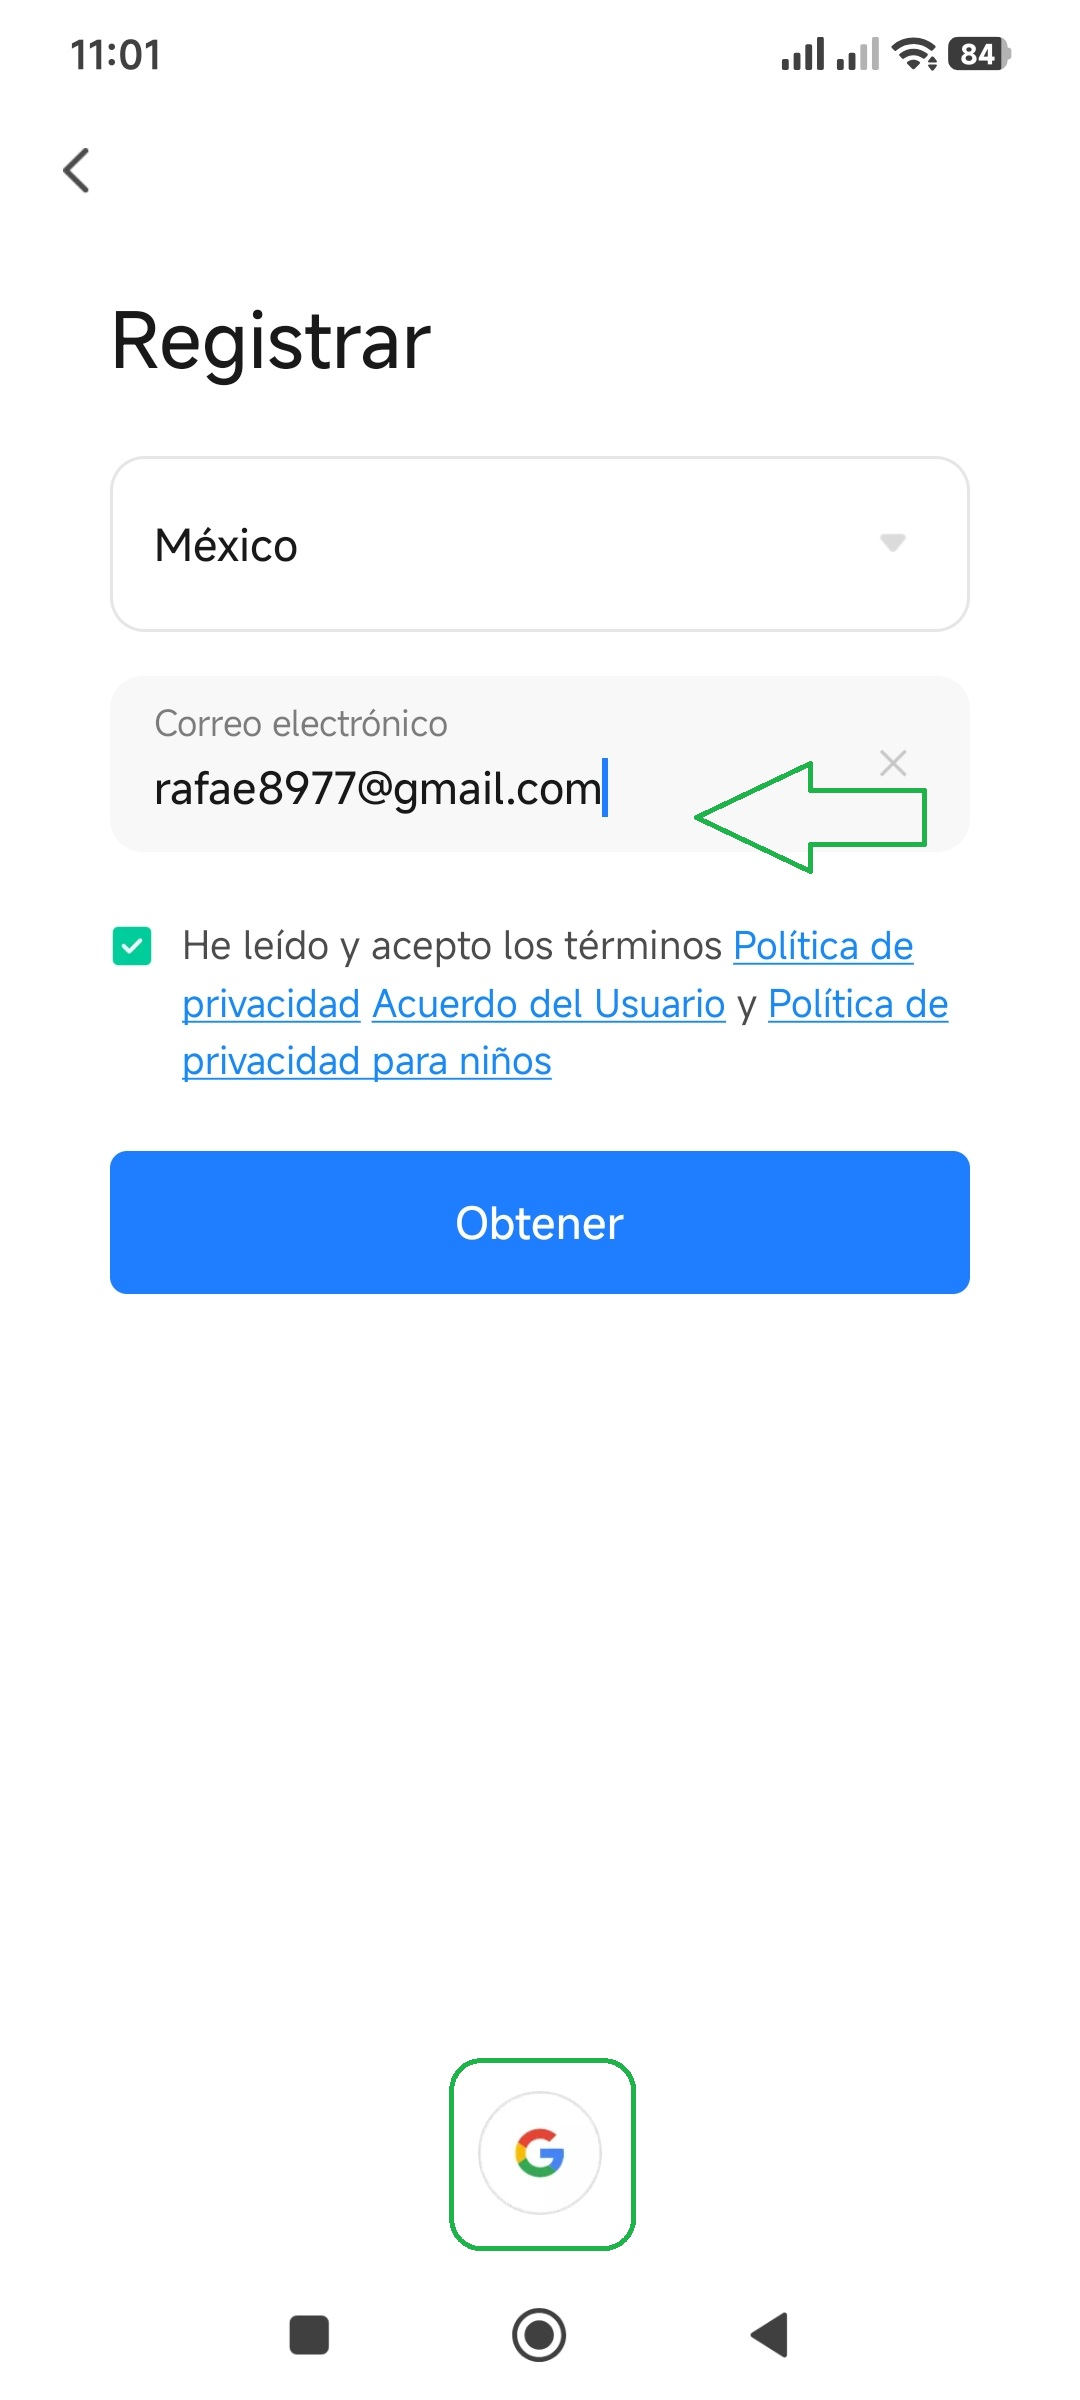
\includegraphics[width=0.4\textwidth]{Paso3.jpeg}
    \end{center}

    \newpage
    %PASO 4
    \item \textbf{Recibir el número de confirmación (Solo para Opción A)}\\
    Le llegará un código de 6 números a su correo electrónico (\textbf{revise} también su carpeta de Spam o Correo No Deseado). \\
    \textbf{Recomendación:} A veces, el primer mensaje tarda un poco en llegar. Si no lo ve de inmediato, le sugerimos \textbf{presionar} el texto azul que dice \textit{Enviar de nuevo} en la pantalla de su celular. Esto hará que el código le llegue al instante.
    
    \begin{center}
        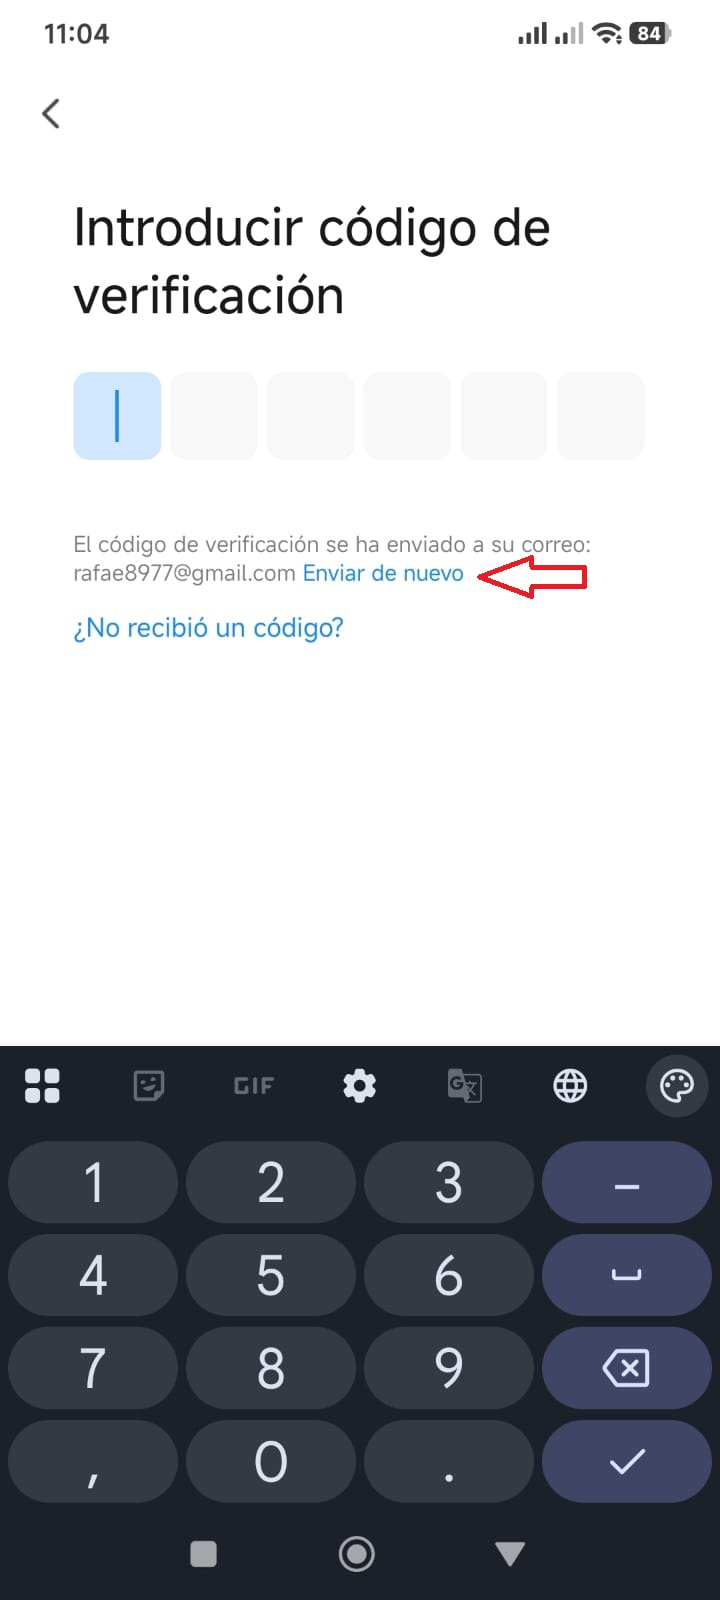
\includegraphics[width=0.4\textwidth]{Paso4.jpeg}
    \end{center}
\end{enumerate}

\newpage
\section*{Permisos de la aplicación}

\begin{enumerate}[label=\textbf{Paso \arabic*:}, leftmargin=*, resume]
    %PASO 5
    \item \textbf{Rechazar las alertas de la reja}\\
    La aplicación le preguntará si desea recibir notificaciones. Por favor, \textbf{seleccione} la opción \textit{No permitir}. Es muy importante rechazar esto para evitar que su celular suene o vibre con avisos molestos cada vez que otro vecino abra la reja.

    \begin{center}
        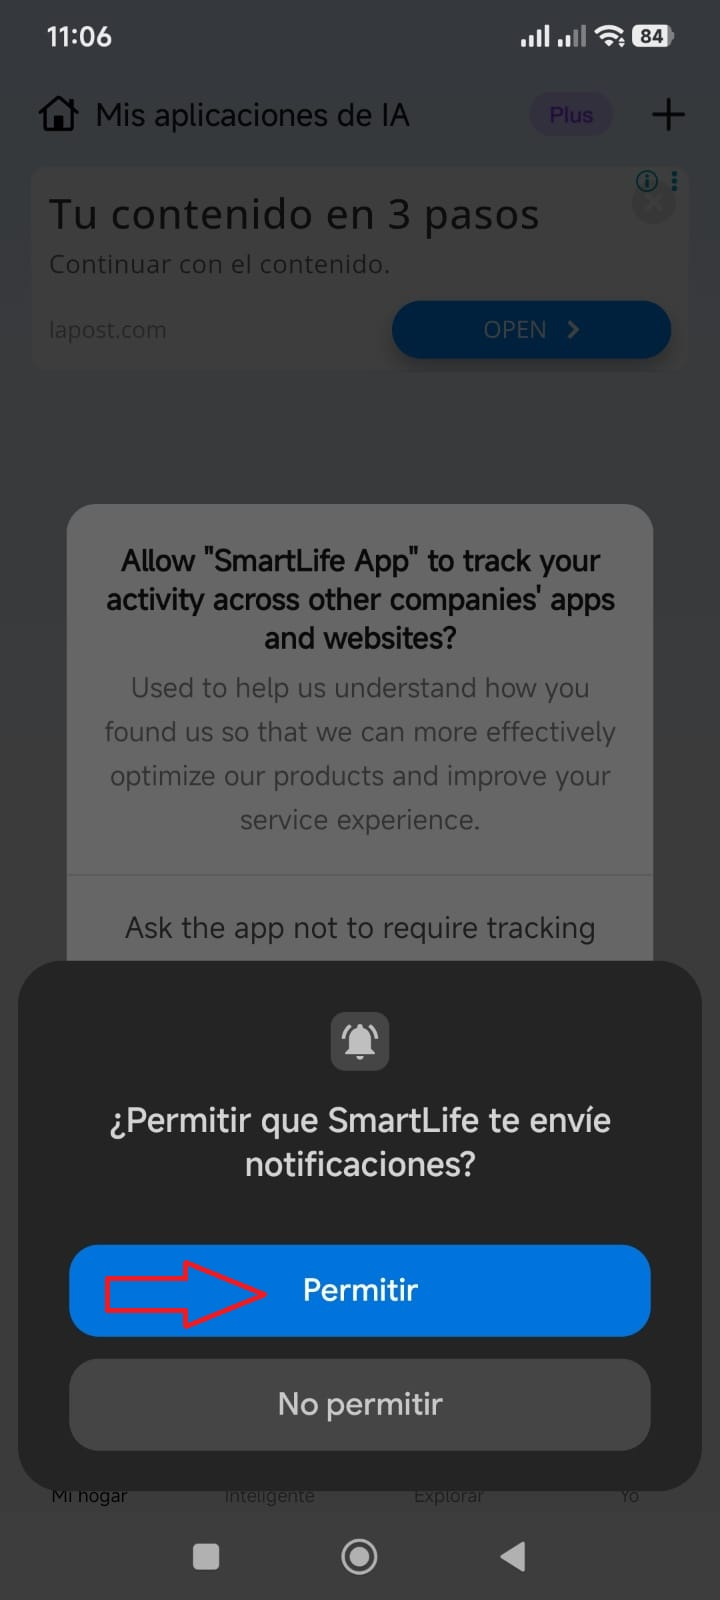
\includegraphics[width=0.4\textwidth]{Paso5.jpeg}
    \end{center}

    \newpage
    %PASO 6
    \item \textbf{Proteger su privacidad}\\
    Si la aplicación muestra un recuadro solicitando rastrear su actividad (\textit{Allow SmartLife App to track...}), \textbf{presione} la opción \textit{Ask the app not to require tracking} (Pedir a la app que no rastree).
    
    \begin{center}
        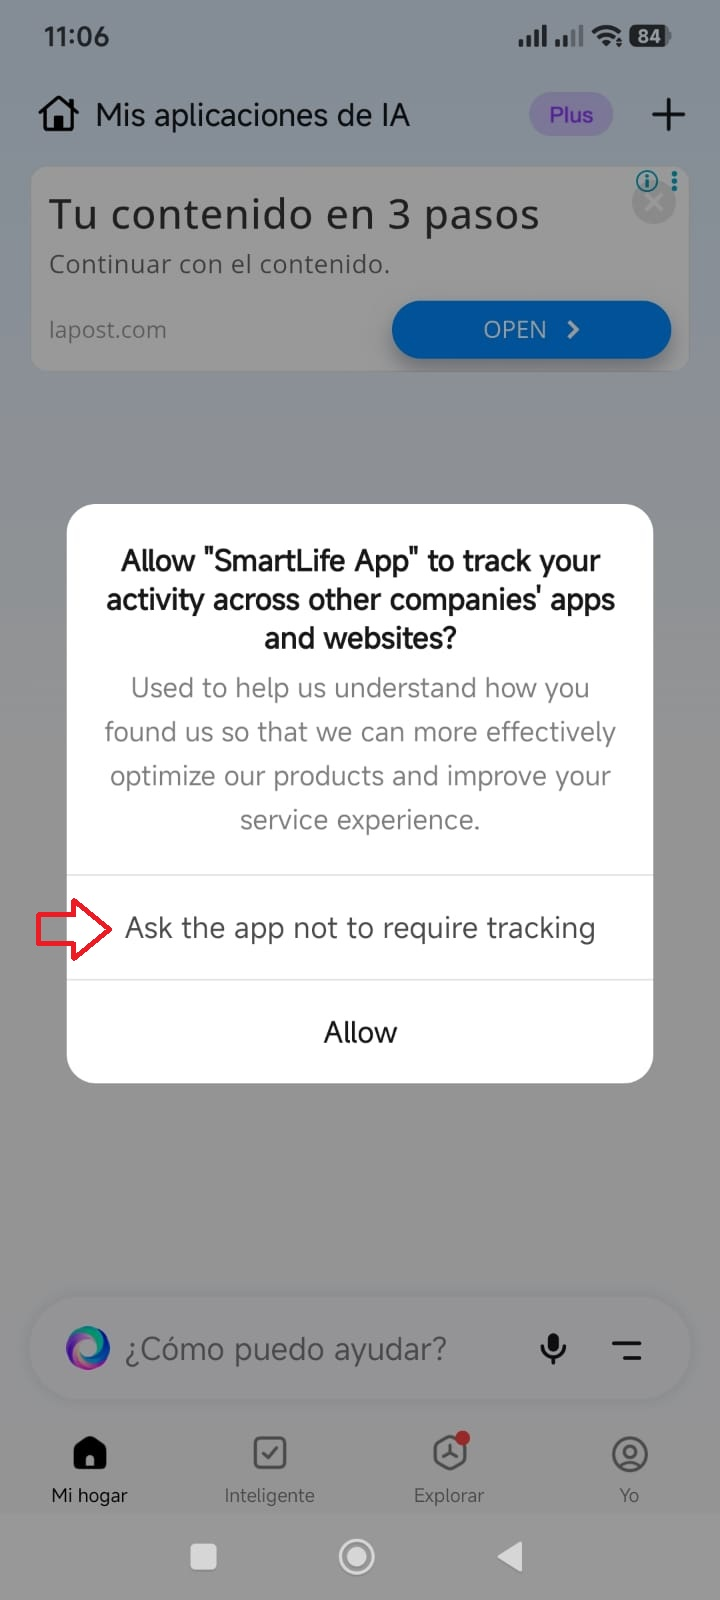
\includegraphics[width=0.4\textwidth]{Paso6.jpeg}
    \end{center}
\end{enumerate}

\newpage
\section*{Crear su casa virtual}

Para recibir el acceso de la reja, la aplicación requiere activar un panel de control personal.

\begin{enumerate}[label=\textbf{Paso \arabic*:}, leftmargin=*, resume]
    
    %PASO 7
    \item \textbf{Ir al menú de su casa}\\
    En el menú inferior de la pantalla, \textbf{seleccione} la opción \textit{Yo}. Posteriormente, \textbf{presione} \textit{Gestión del hogar}. En la siguiente lista, \textbf{elija} la primera opción que dice \textit{Mi hogar ..} (\textbf{evite presionar} \textit{Crear una familia}).
    
    \begin{center}
        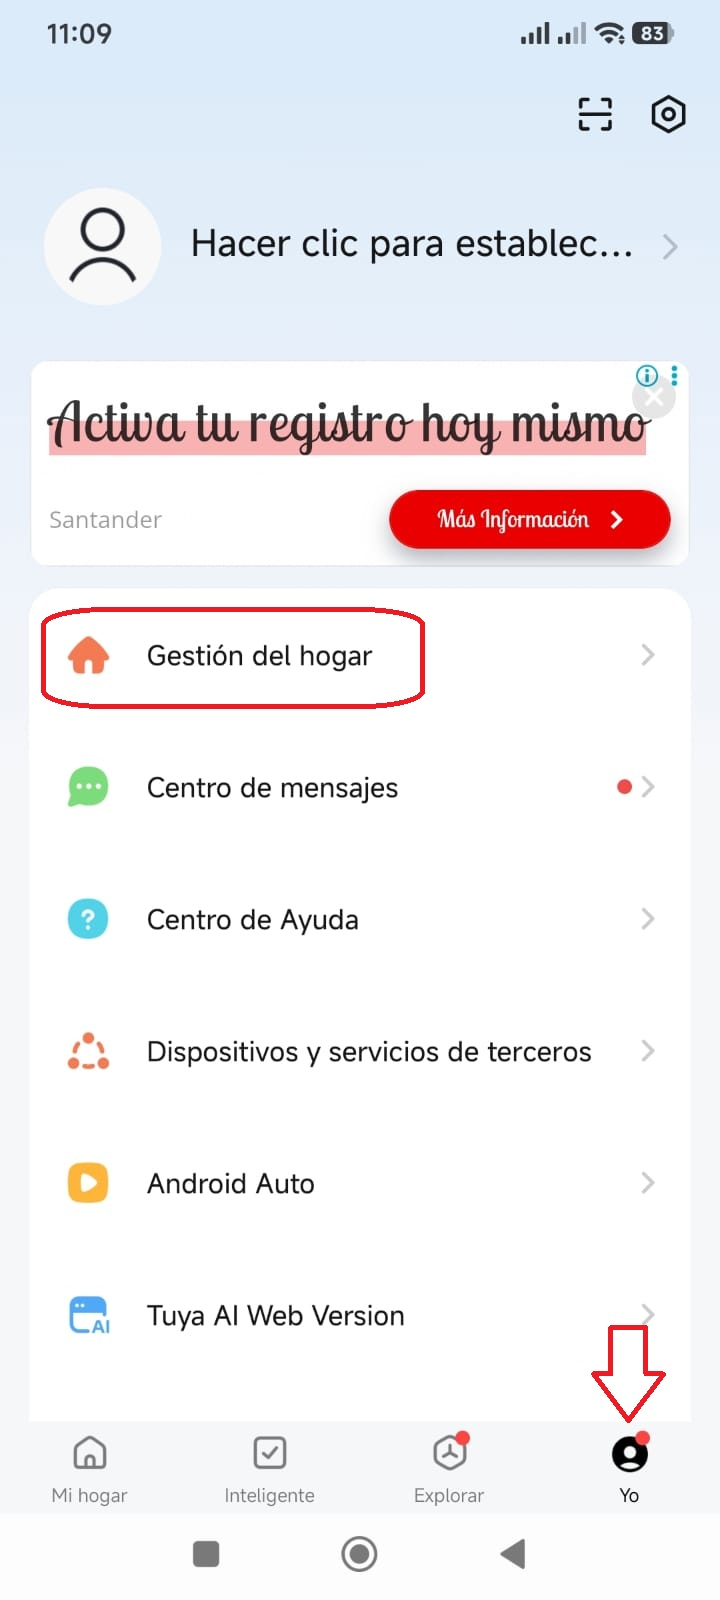
\includegraphics[width=0.4\textwidth]{Paso7.jpeg}
        \hspace{0.5cm}
        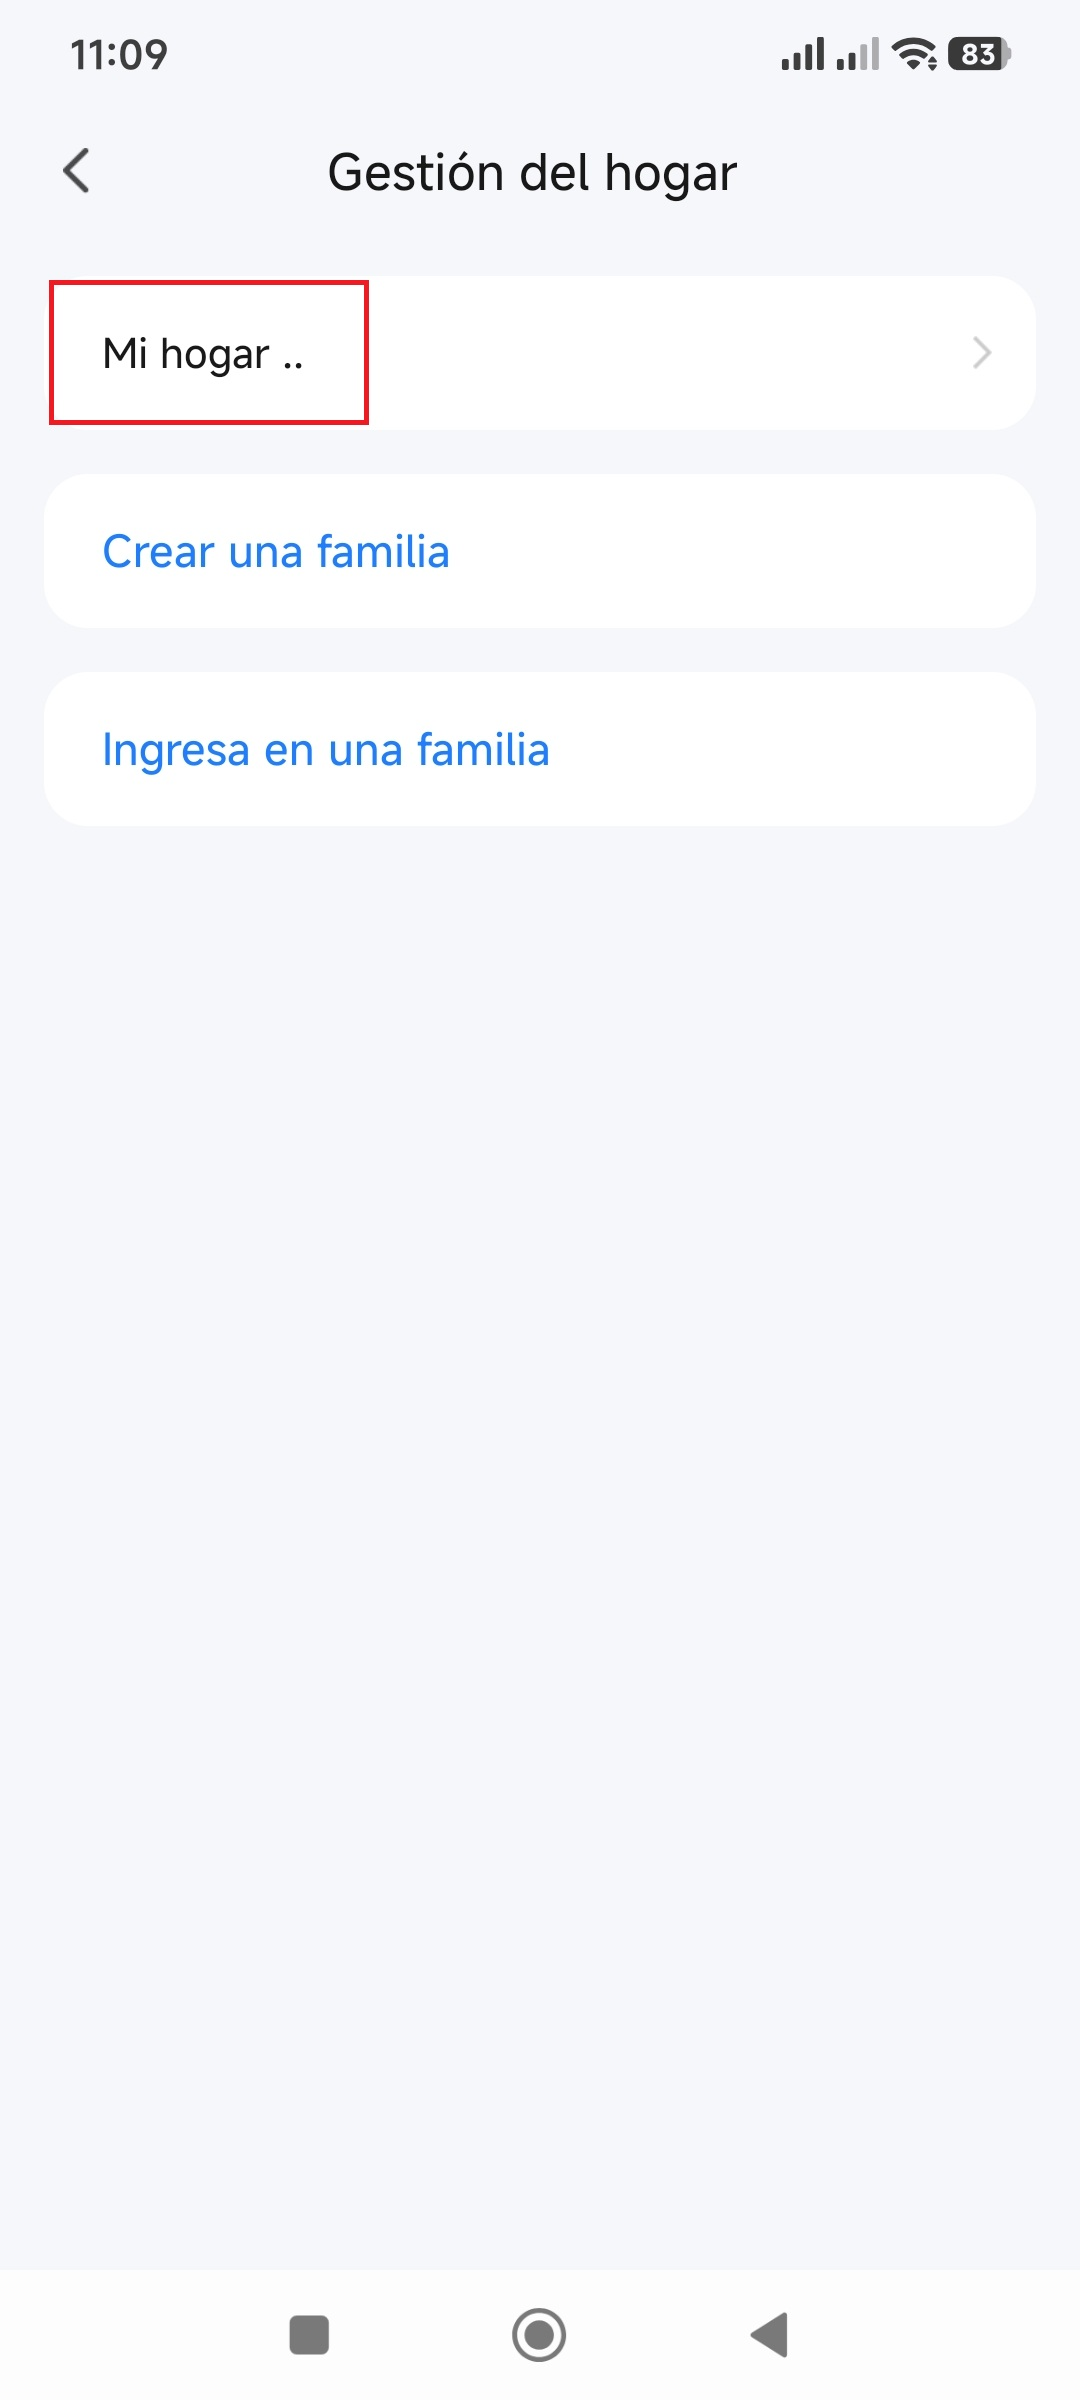
\includegraphics[width=0.4\textwidth]{Paso9.jpeg}
    \end{center}
    
    \newpage
    
    %PASO 8
    \item \textbf{Ponerle nombre a su casa}\\
    En el campo \textit{Nombre del hogar}, \textbf{escriba} únicamente \textit{Mi Casa}. Puede ignorar el resto de las opciones (\textit{Salón, Dormitorio, etc.}) y \textbf{presione} directamente \textit{Guardar} en la esquina superior derecha.
    
    \begin{center}
        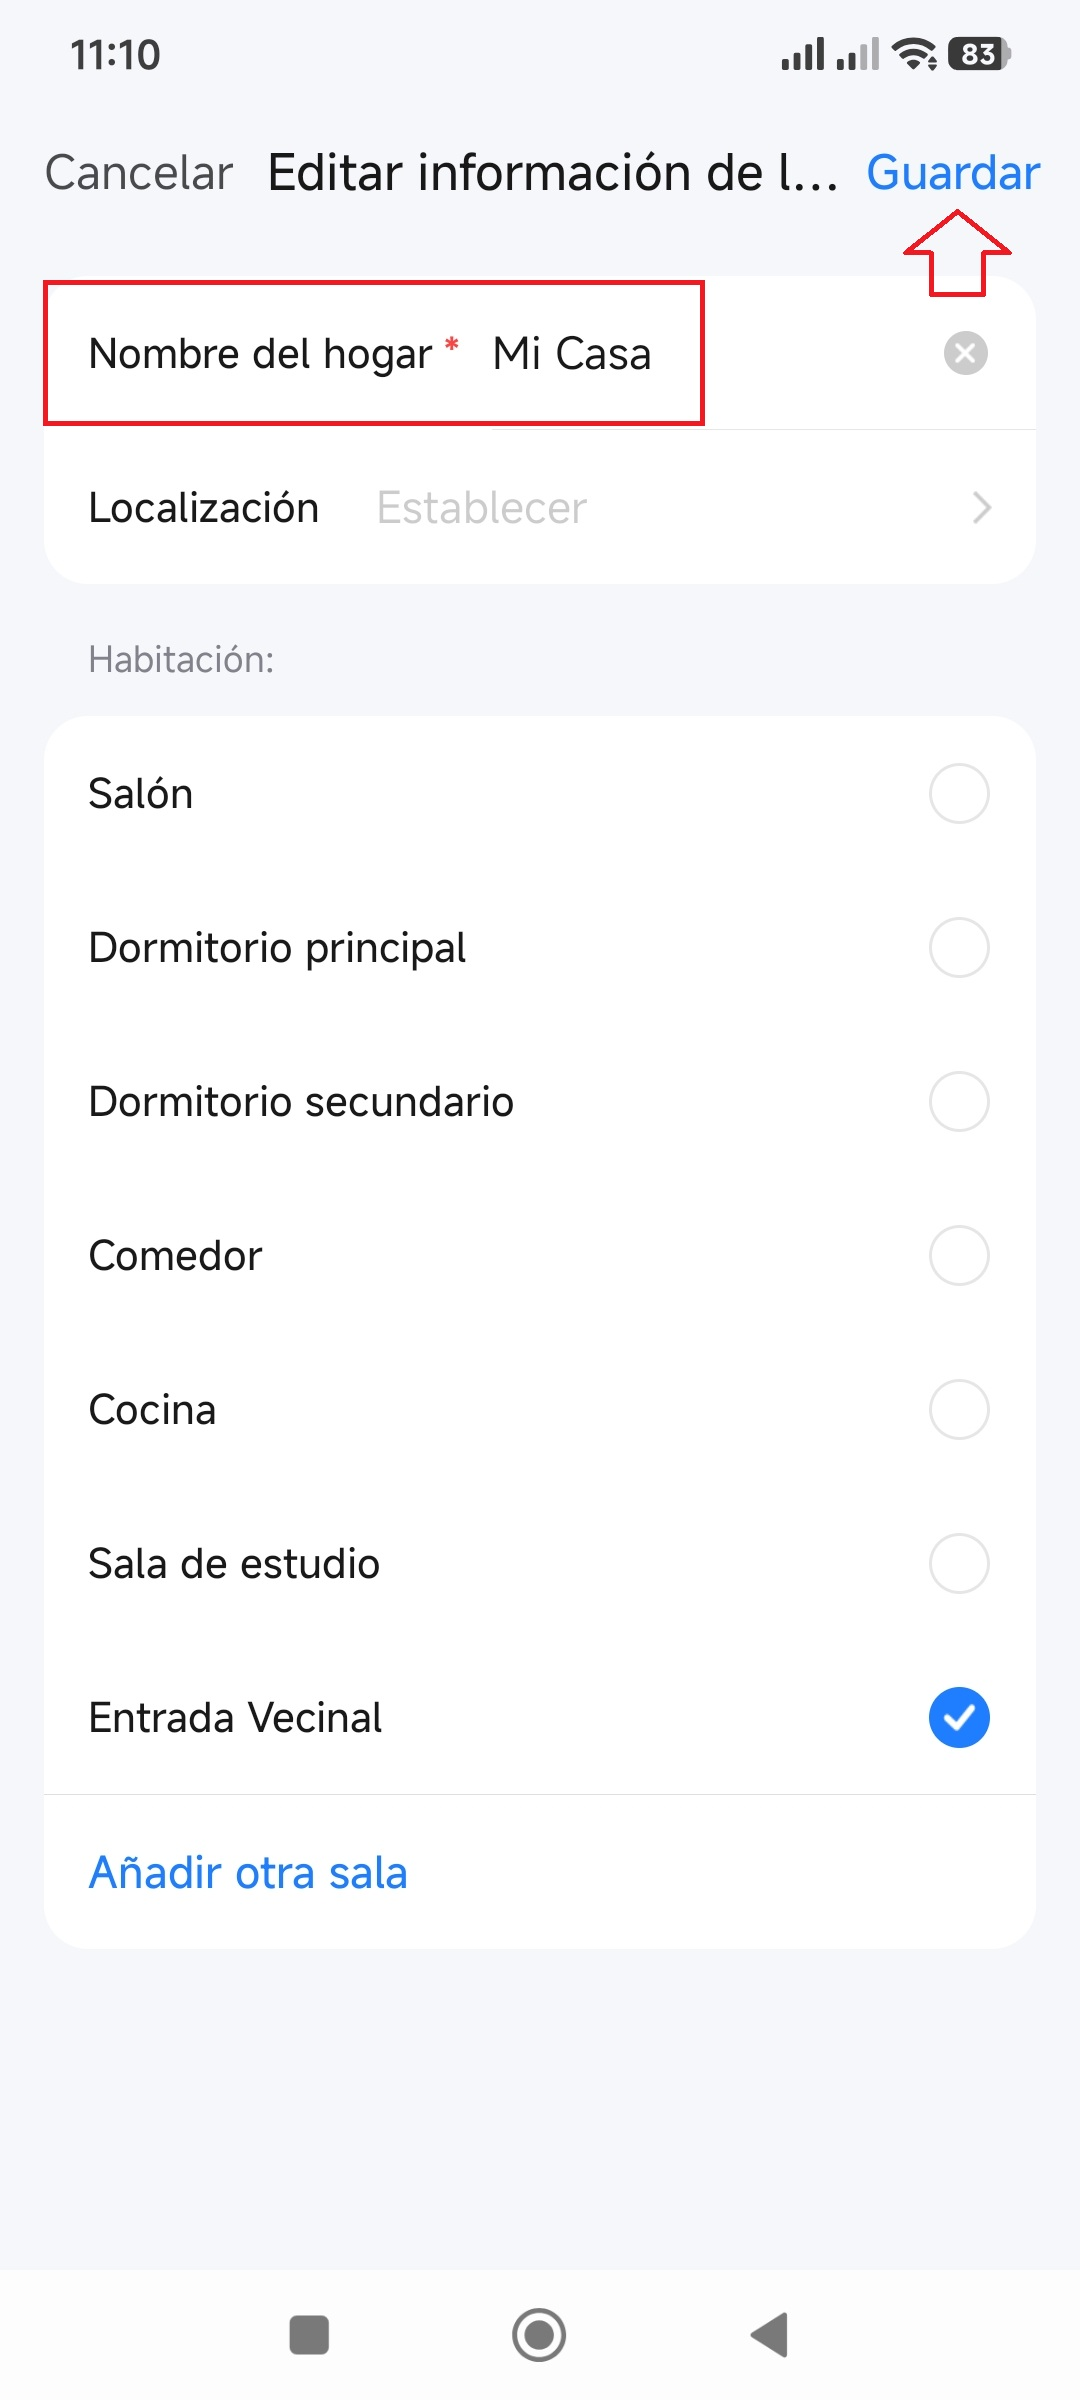
\includegraphics[width=0.4\textwidth]{Paso10.jpeg}
    \end{center}
\end{enumerate}

\newpage
\section*{Recibir el control de la reja}

\begin{enumerate}[label=\textbf{Paso \arabic*:}, leftmargin=*, resume]
    
    %PASO 9
    \item \textbf{Buscar el botón del portón}\\
    \textbf{Regrese} a la pantalla principal (\textit{Mi hogar}). En la parte superior, \textbf{presione} el pequeño menú desplegable junto al nombre de su casa y \textbf{seleccione} \textit{Gestión de dispositivos}.
    
    \begin{center}
        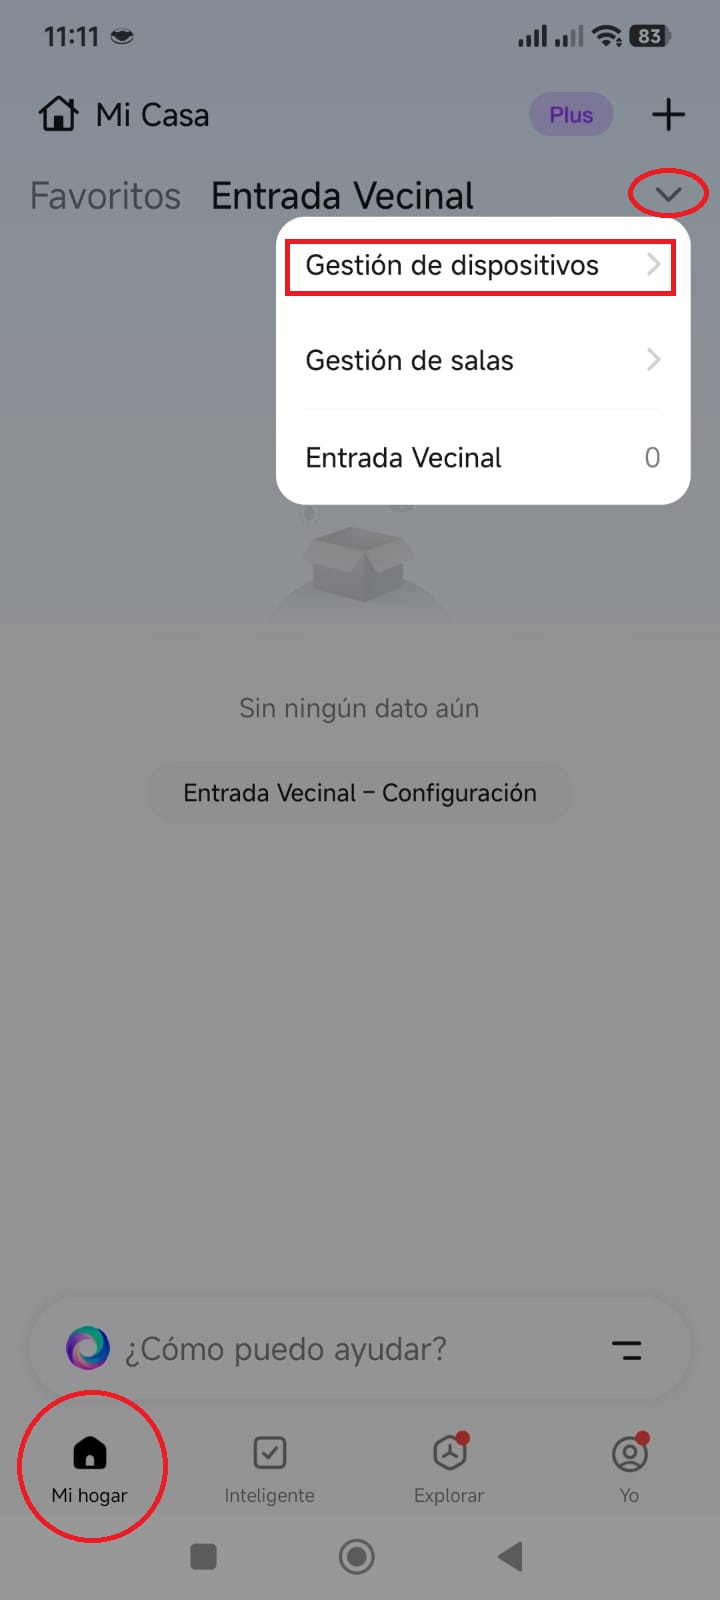
\includegraphics[width=0.4\textwidth]{Paso11.jpeg}
    \end{center}
    
    \newpage
    
    %PASO 10
    \item \textbf{Dar permiso de Bluetooth (Necesario)}\\
    La aplicación solicitará \textit{Acceso a dispositivos cercanos} (Bluetooth y Red). \textbf{Presione} el botón azul \textit{Continuar} y posteriormente \textit{Permitir}. Sin este permiso, la aplicación no podrá enviar la señal a la antena de la reja.
    
    \begin{center}
        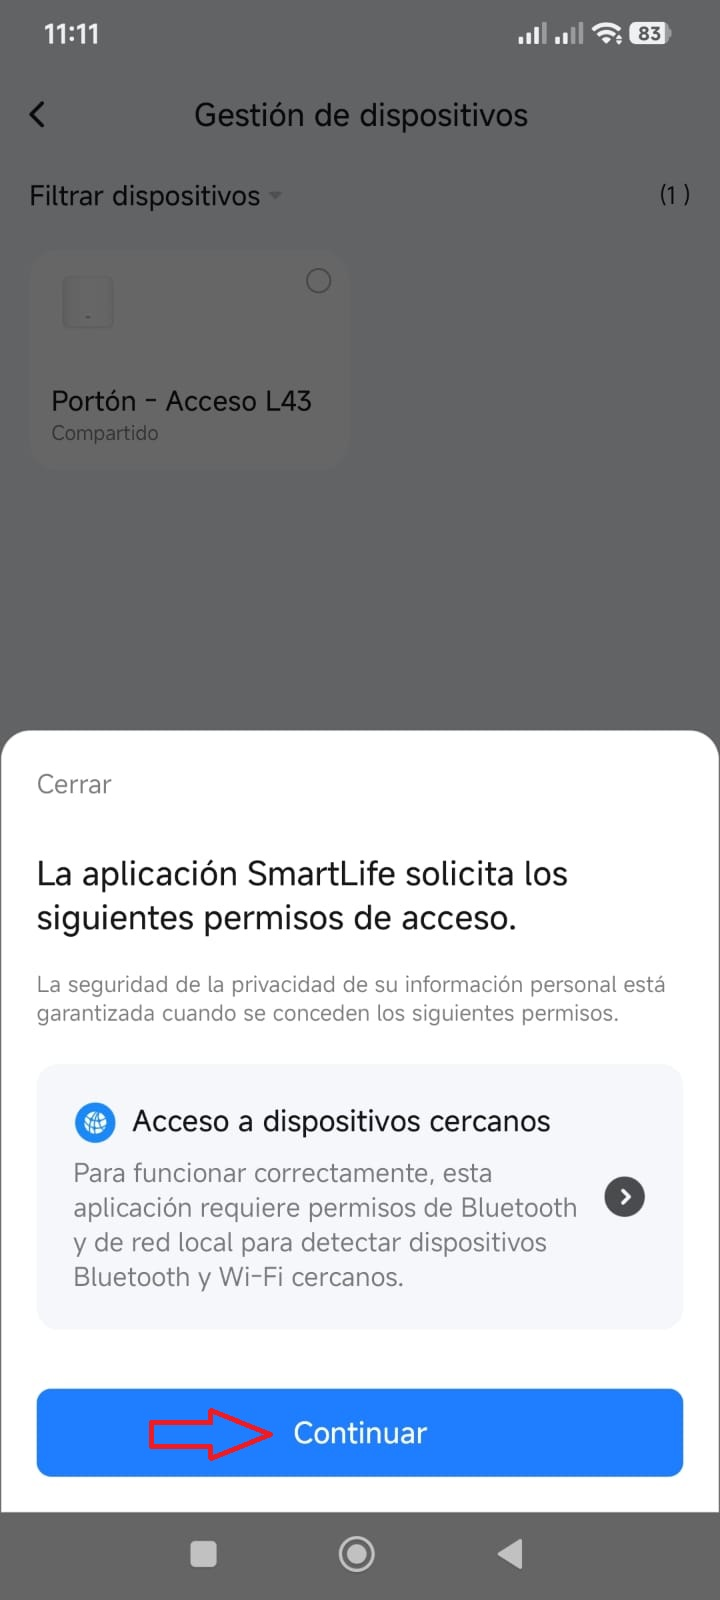
\includegraphics[width=0.4\textwidth]{Paso12.jpeg}
    \end{center}

    \newpage
    
    %PASO 11
    \item \textbf{Colocar el botón en su pantalla}\\
    En la pantalla aparecerá el acceso autorizado. \textbf{Toque} el pequeño círculo a la derecha para que se marque con una palomita azul y \textbf{presione} \textit{Agregar al hogar} en la parte inferior.
    
    \begin{center}
        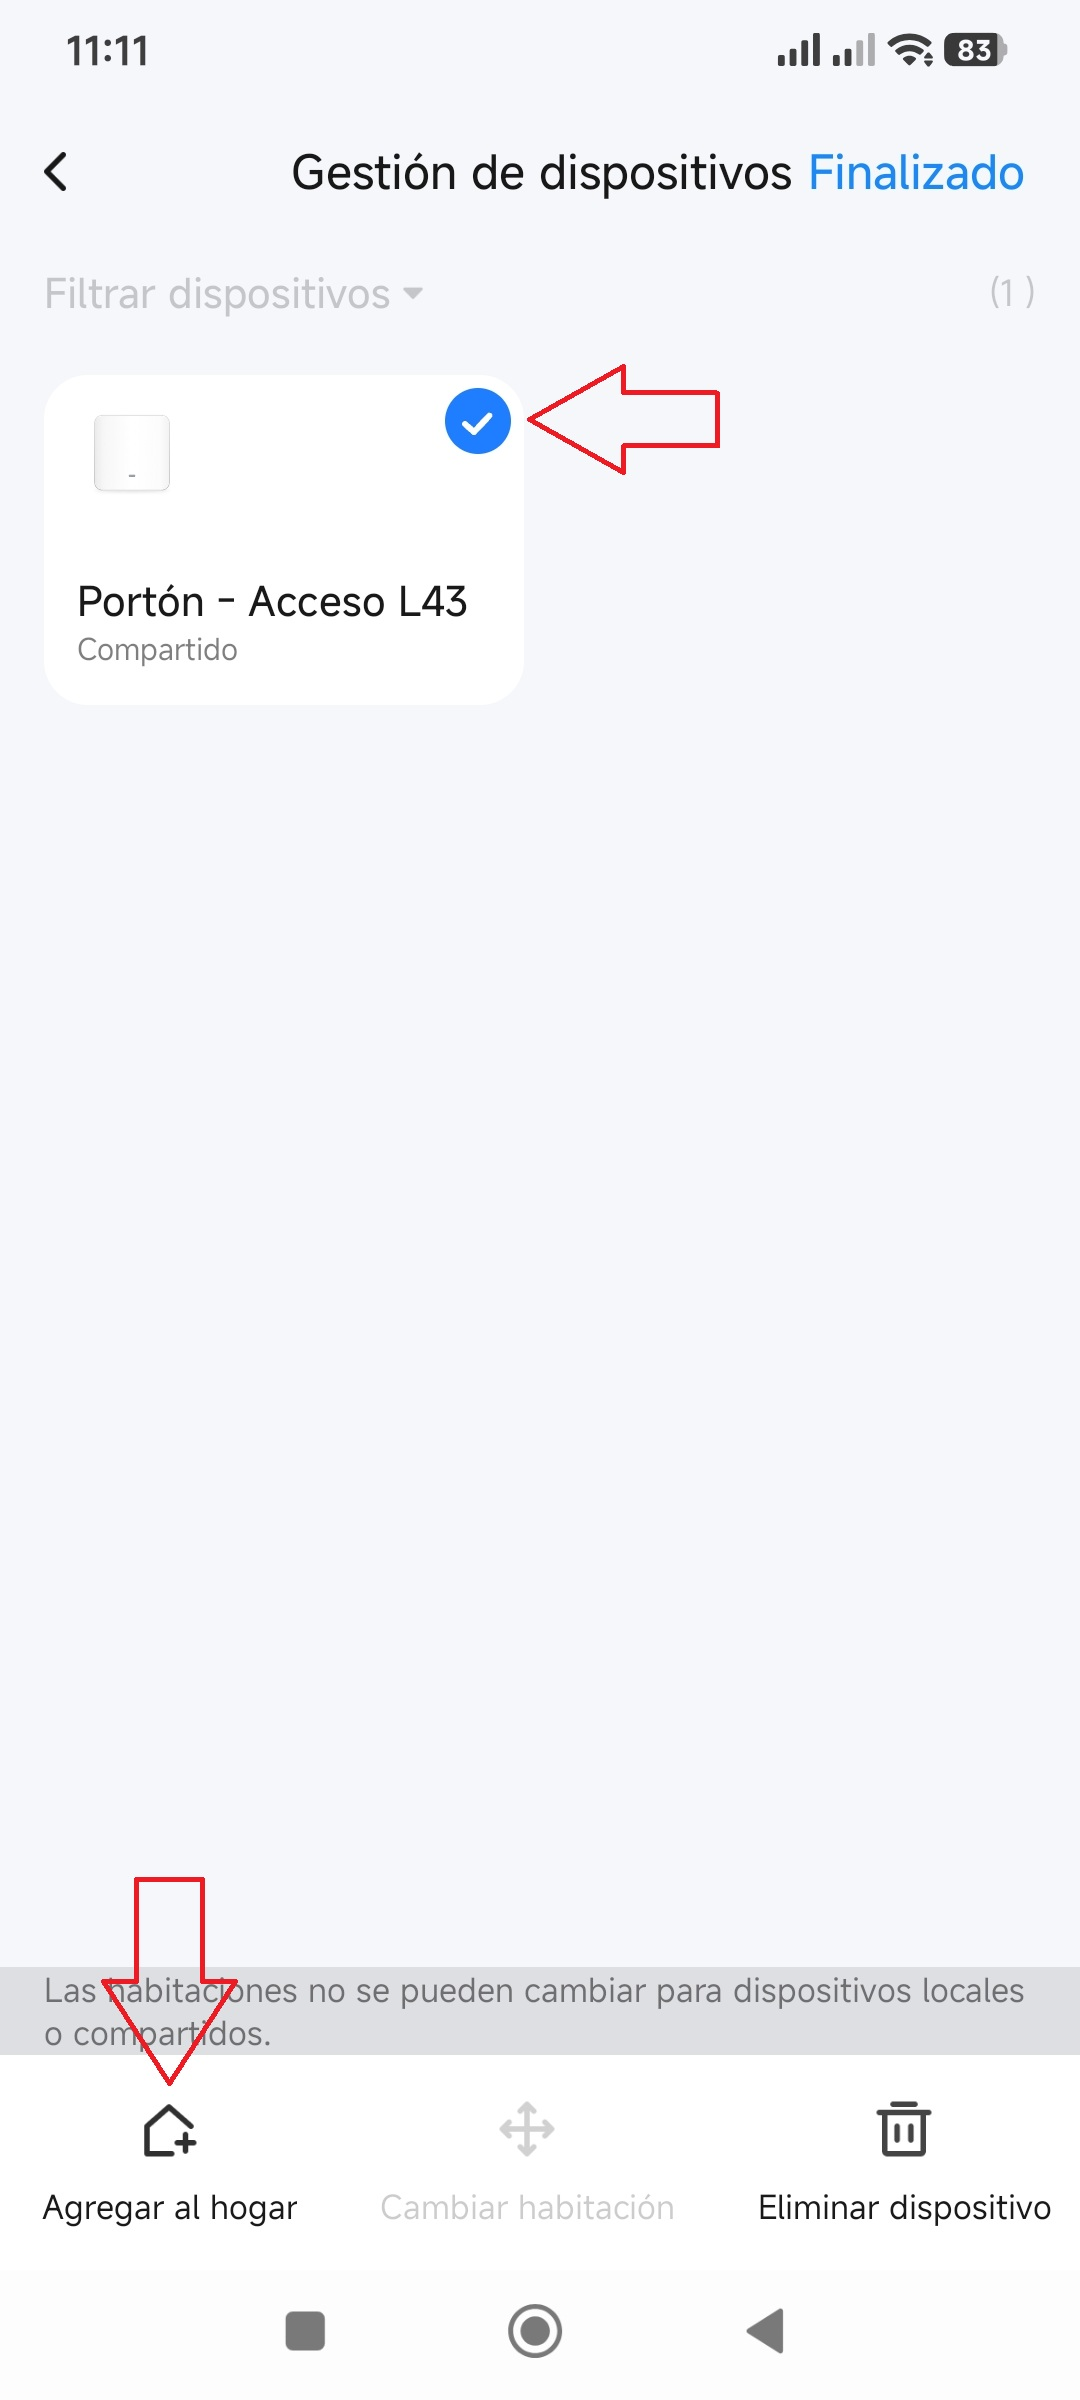
\includegraphics[width=0.4\textwidth]{Paso13.jpeg}
    \end{center}
\end{enumerate}

\newpage
\section*{¡Ya puede usar su celular como control!}

\begin{enumerate}[label=\textbf{Paso \arabic*:}, leftmargin=*, resume]
    
    %PASO 12
    \item \textbf{¡Proceso Concluido!}\\
    El botón para controlar su reja ya está listo en la pantalla principal de su aplicación. Para abrirla, simplemente \textbf{presione} el pequeño botón de encendido que aparece a la derecha, o \textbf{toque} el nombre del portón para entrar y ver un botón mucho más grande.
    \begin{center}
        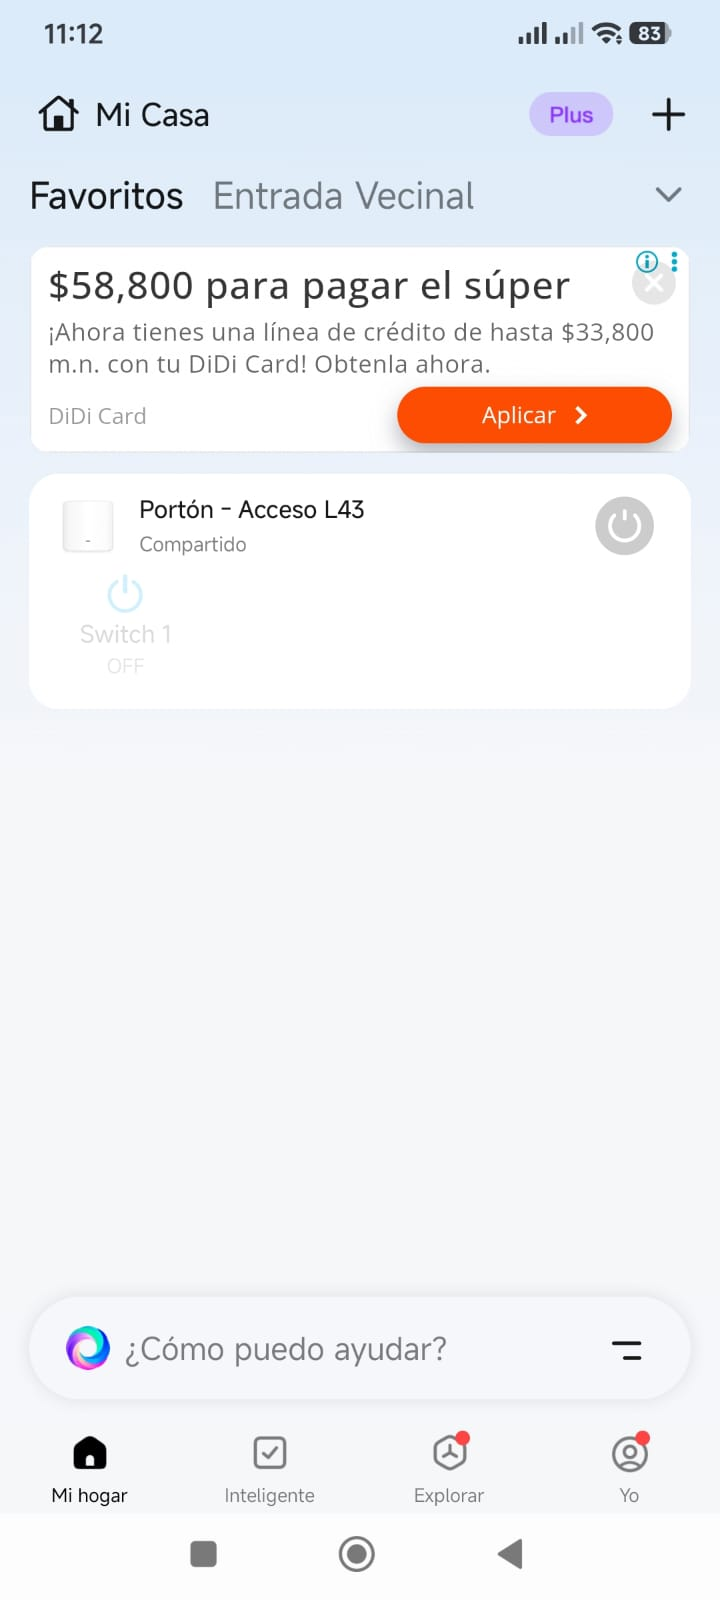
\includegraphics[width=0.4\textwidth]{Paso14.jpeg}
        \hspace{0.5cm}
        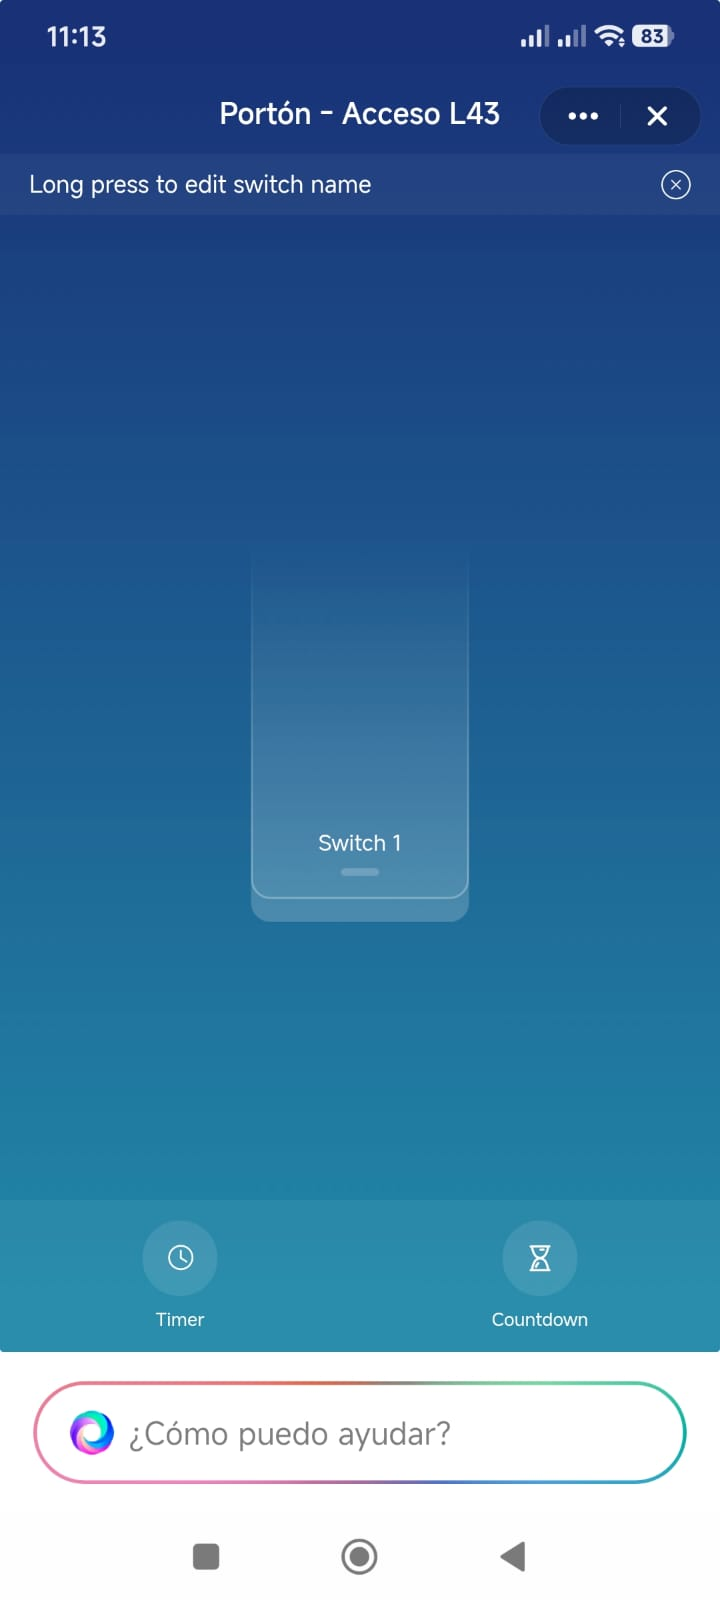
\includegraphics[width=0.4\textwidth]{Paso15.jpeg}
    \end{center}
\end{enumerate}

\vspace{1cm}
\begin{nota}
    Si presentó algún error durante este proceso o la aplicación le indica que no tiene dispositivos compartidos, \textbf{asegúrese} de haber iniciado sesión con el correo electrónico correcto. Para asistencia técnica adicional, \textbf{contacte} a la administración.
\end{nota}

\end{document}